%! TEX root = **/000-main.tex
% vim: spell spelllang=en:

\section{DDI}%
\label{sec:ddi}

\subsection{Architecture}%
\label{sub:ddi-arch}

\paragraph{Inputs:} First we tried with only words as inputs, but giving also words in
lower case, lemmas and PoS improved the model quite a lot (around 10\% accuracy improvement).
Additionally, we decided to add also add the syntactic function of the nodes since it was easy
to add and seemed to provide marginally better results (\approx \, 3\% accuracy increase).
We also tried to adff suffix and prefix information, but it performed worse.

\paragraph{Embeddings:} we tried various embeddings and combinations of them. We found that
using the \texttt{TokenPositionEmbedding} for all the inputs and complement it with the
embedding of words and lowercase words from GloVe worked best in our trials. Just using
the TokenPositionEmbedding, we got an increase of from 45\% to 55\% and when combined with gloVe
we reached 62\%.

\paragraph{Concatenation:} since we had different inputs, we had to merge the different embeddings
together at some point. This presents two main challenges: when in the model pipeline should we
merge them, and what operation should we use. %TODO

\paragraph{CNN, RNN and LSTM} we tried various configurations of CNN, RNNs and LSTMs:

\begin{itemize}
\item \textbf{CNN}: We tried 1 and 2 convolutional layers with various sizes, the results
obtained did not surpass the 52\% accuracy mark on the test set.

\item \textbf{RNN}: RNNS

\item \textbf{Bidirectional LSTM:} this was the best performing method of the ones we tried and part
of our final model, which achieved 67.0\% accuracy on the train dataset. Using plain LSTM
without bidirectionality,
we obtained results
\end{itemize}

\paragraph{TransformerBlock}: using \texttt{TransformerBlock} we got the worst results from the
different methods we tried (36\% accuracy). This was probably because our embeddings were not suited

\paragraph{BERT}: we tried using BERT, but unfortunately, we did not manage to properly incorporate
into a keras as part of a model.


\subsection{Input information}%
\label{sub:ddi-input}

For the input, as stated before, we used:
word, word lowercase, lemma, PoS tag and the node syntactic function (rel).
The latter was added to Codemaps and Dataset since it was not generated by the default code.

\subsection{Code}%
\label{sub:ddi-code}

\subsection{Experiments and results}%
\label{sub:ddi-experiments}

\begin{figure}[H]
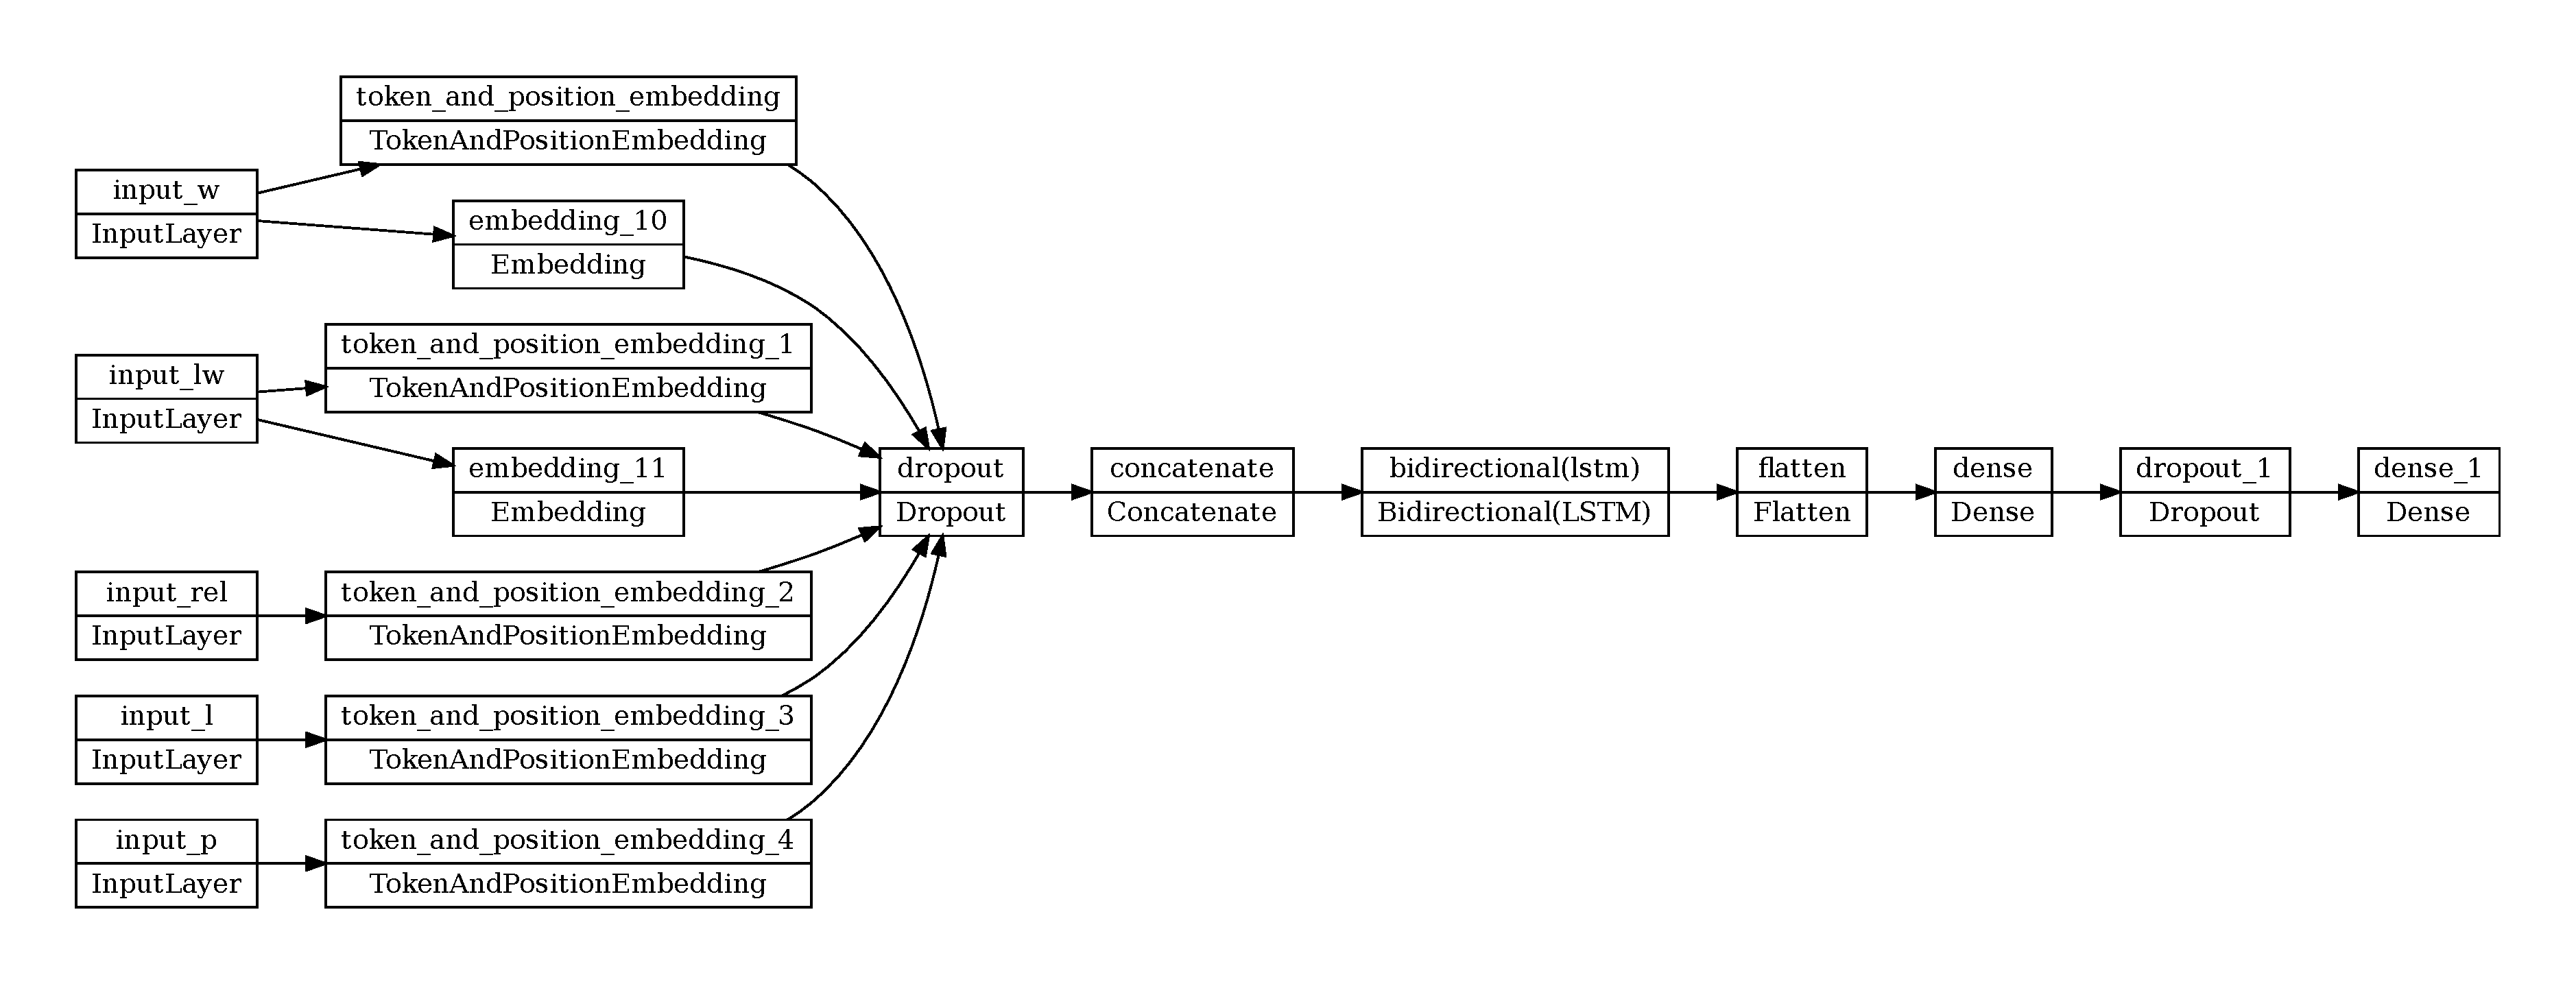
\includegraphics[width=\linewidth]{model_ddi}
\caption{Final DDI Architecture}
\end{figure}